\subsection{Data}
\subsubsection{Regression data}
We have generated the data for the regression problem using the Franke function \citep[p. 13]{frank}.
\begin{align}
\begin{split}\label{eq:franke}
    f(x, y) = &\frac{3}{4} \exp\left( -\frac{(9x - 2)^2}{4} - \frac{(9y - 2)^2}{4} \right) \\
    + &\frac{3}{4} \exp\left( -\frac{(9x + 1)^2}{49} - \frac{(9y + 1)^2}{10} \right)  \\
    + &\frac{1}{2} \exp\left( -\frac{(9x - 7)^2}{4} - \frac{(9y - 3)^2}{4} \right)  \\
    - &\frac{1}{5} \exp\left( -(9x - 4)^2 - (9y - 7)^2 \right)
\end{split}
\end{align}
\begin{align}\label{eq:franke_noise}
    f^*(x,y) &= f(x, y) + \frac{3}{10} \mathcal{N}(0, 1)
\end{align}
The Franke function is defined by Eq. \ref{eq:franke}, on the domain $[0, 1]^2$. 
In order to challenge the models, and test them for weaknesses such as overfitting, we have added a stochastic noise term to the function, as can be seen in Eq. \ref{eq:franke_noise}, where $f(x,y)$ is as defined in \ref{eq:franke}.
For the Franke data, we use 101 data points along each axis, for a total of 10201 data points (i.e. $101^2$).
The Franke function with noise is plotted in Fig. \ref{fig:franke_noise}.
All further references to the Franke function in the results and discussions refers to the Franke function with noise (Eq. \ref{eq:franke_noise}).

\begin{figure}[h!]
\centering
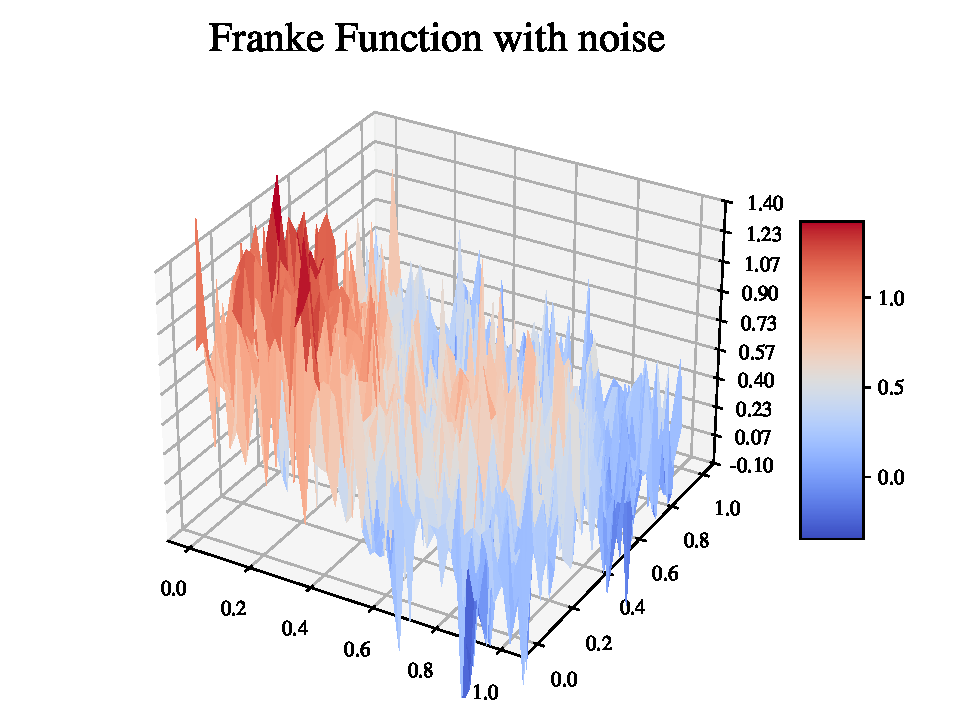
\includegraphics[width=1\linewidth]{project_1/figures/figures_in_report/franke_func_noise.pdf}
\caption{The Franke function for $x,y \in [0,1]$ with added noise term: $(3/10) \mathcal{N}(0, 1)$.}
\label{fig:franke_noise}
\end{figure}

\subsubsection{Classification data}
For the classification problem, we test the models using the Wisconsin breast cancer diagnostics data set \cite{breast_cancer_wisconsin}.
The data set contains 30 different features of digitized images computed from a fine needle aspirate of a breast mass, describing the characteristics of the cell nuclei in the images.
It also contains a column describing the diagnosis of the breast tissues; malignant or benign.
There are 569 patients registered in the data set, with no missing data.
357 of the patients have diagnosis benign, while 212 are malignant.
More details about how the data is produced is available in \textcite{Street1993NuclearFE}.

\subsubsection{Data handling}
To make sure the models learn the underlying structure of the data, instead of just copying the set of data points, we split our data in a training set and a test set.
This is common practice in machine learning problems, and is known as \textit{train-test split}.
By setting aside 30\% of the data as test data, we make sure that the model can, after being trained on the training set, predict new data points it has never seen before with a reasonable accuracy.
When presenting accuracy and error numbers in the results used for comparing models, we use the measures on the test data unless indicated otherwise.

The Franke data has input in the range $[0, 1]$ for both variables.
This means that min-max scaling (Eq. \ref{min-max}) would have no effect on the data, as it is already min-max scaled.
We tested using standard scaling (Eq. \ref{standardize}), however this gave worse results, hence we decided on not scaling the data.
% %Our theory for why min-max scaling (not scaling) gave the best result, is that \gaute{jeg vet da faen, jeg...}

For classification, we also tested both min-max scaling (Eq. \ref{min-max}) and standard scaling (Eq. \ref{standardize}), described in section \ref{sec:scale}.
When testing logitstic regression and the neural networks, it became clear that min-max was superior in both cases.

\subsection{Implementation of the models}
\subsubsection{Linear regression}

For linear regression, we reuse our earlier implementation of ordinary least squares regression and ridge regression for the Franke data set. A more detailed discussion of this implementation can be found in \textcite{project1}.

\subsubsection{Neural network}\label{sec:nn_imp}

We implement a flexible neural network class in our code, enabling it to work for both classification and regression problems, with different structures, cost functions, activation functions and learning rate algorithms.
Having cost functions, number and size of layers, activation functions, mini-batch sizes and gradient descent methods as arguments when setting up the class, allows us to easily explore different models.
We input the network shape as an array of integers, where the first element represents the input shape, the last element represents the output shape and the rest represent the sizes of the hidden layers.
The argument for mini-batch sizes for SGD defaults to normal gradient descent if set to 0.

While having implemented backpropagation with manual derivatives to find the gradients, we mainly use the \texttt{grad} function from \texttt{JAX} \cite{jax2018github} to get the gradients more efficiently.
Our tests includes a control check that the gradients form \texttt{JAX} and our manual gradients are identical.

The initialization of the parameters is done with a normal distribution with expectation 0 and standard deviation 1.
While there exists more advanced initialization schemes (see section \ref{sec:NN_init}), we decided not to spend time implementing these.
This is due to the fact that we are using several different activation functions, and many of the initialization schemes are specialized at being good for one particular activation function.
We also use relatively simple neural networks structures with a relatively small amount of hidden layers and nodes, meaning it does not cost us much extra time or computation power needing to spend a few more iterations training them.

When using SGD, we have only one update in each epoch matching the first view in the discussion in section \ref{sec:gd}.
We make the mini-batch by making a list of all the indices of data points, shuffling it using \texttt{NumPy}'s shuffle method \cite{NumPy-Array}, and selecting the first $m$ indices (where $m$ is the size of the mini-batch).
Before running the parameters and gradients through the adaptive learning rate algorithm of choice, we flatten/ravel the parameter object into an array from \texttt{NumPy} \cite{NumPy-Array}, enabling us to perform mathematical operations on the entire set of parameters at once in an effective way.
After updating the the parameters, we reshape them into the original structure.

Due to neural networks sometimes taking long to train, and the stochastic nature in initialization and mini-batches, we have implemented methods to save and load a network.
This is done through methods in the neural network class, and all the required information about the networks i stored as a \texttt{json} file.
We also made it possible to save a half-trained networks, and resume the training after loading it, including storing the epoch number.
Since the networks in this paper are relatively small and fast to train, we did not actively use these methods, however they will be useful in further expansions and applications of this code base.

\subsubsection{Logistic regression}

As explained in the theory, a logistic regression model is in essence a neural network with no hidden layers and the sigmoid function as activation.
Our implementation is inspired by this; we make the layers similarly as in the neural network code, just limited to only having one layer.
Furthermore, we implemented cross entropy as the cost function inside the class, adding an $l_2$ regularization part to it, with parameter $\lambda$ defaulting to 0.

We initiate our weights and biases using a normal distribution with expectation 0 and standard deviation 1.
While we could have used specialized initiation schemes as described in section \ref{sec:NN_init}, we reached convergence fast enough with the naive approach to not prioritize that.
We use \texttt{JAX} \cite{jax2018github} to get the numerical gradients while training the model, and implement our mini-batch code as in the neural network case.
We also implement custom functions for flattening and reshaping the weights and biases, but we use different functions for logistic regression than for neural networks, since we can make them much simpler and somewhat faster as logistic regression has an easier structure.

\subsection{Exploration and testing}
\subsubsection{Exploration of the properties of a neural network}

For the Franke function data, we use mean squared error as our cost function. For the classification case, i.e. the cancer data, we opt for binary cross entropy as our cost function.

As a measure of performance, $R^2$ is used for the Franke function data, while accuracy is used for the Wisconsin breast cancer data set during the exploration. 
In the end, we calculate accuracy, recall, precision, and F-score for the classification case. 

Sigmoid is always utilized as the activation function in the final layer for the classification. 
For the regression (Franke data), we do not apply any activation function in the final layer.
Formally, our activation function is the identity.

First, we want to find a good optimizer to use for the exploration of the other moments. 
To do this, we initialize our neural network model with a learning rate of 0.005 and two hidden layers of size 4 and 8 respectively. 
We train the models for 300 epochs through the entire exploration process, before increasing it in the final selected model. 
We use ReLU as activation function i both the hidden layers.
For the Cancer data, sigmoid is used at the final layer, whereas for the Franke function data, we do not use an activation (i.e. identity). 
We use a batch size of 200 and 1000 for the Cancer data and the Franke function data respectively.

We use the following optimizers: constant, momentum, Adam, Adagrad with momentum and RMSprop. 
A sixth optimizer, Adagrad, is also implemented, but performs so badly on the neural network for the regression case that it surpresses the visibility in the plots. 
We therefore remove it completely. 
We train six different models, one for each of the optimizers, for the two different data sets. 
We choose the optimizer that performs best for use in further explorations of the neural network. 

Next, we explore the structure of the network. We choose to test two and three hidden layers with each having the size 8 or 24. 
This amounts to 12 different combinations. 
These values were chosen after trial and error.
With the exploration taking quite a lot of computation time, this seems like a good set of values to explore the properties of the structure of the neural networks. 
We find the network structure that produces the best performing model in terms of accuracy or $R^2$, and keep this accuracy for further exploration. 

After that, we study the activation functions of the hidden layers. At the final layer we choose to always use sigmoid for the classification problem and the identity function for the regression problem. 
Three different activation functions is tested: ReLU, sigmoid, and leaky ReLU. For two hidden layers, these three activation functions can be combined in eight ways. Here, as in the previous steps, we find the best set of activation functions for each problem and continue with these. 

Furthermore, we conduct a grid search for the best combination of initial learning rate and batch size. For both problems, we test the following learning rates: \{0.01, 0.001, 0.0001\}. 
For the regression problem, we test the batch sizes \{1000, 3000, 5000\}, whereas \{100, 200, 300\} are tested in the classification problem. 
This is simply because we have a lot more data in the regression problem, seeing as the data is generated from the Franke function expression. This grid search is conducted for the three best-performing optimizers from the first step. 
A combination of initial learning rate and batch size is chosen for each of the three optimizers and brought to the final stage of the exploration. 

For the final step, we train the three models for a total of 500 epochs, one for each optimizer. All three use the network structure and set of activation functions found to be the best. They each have their own best combination of learning rate and batch size. 
We find the best model among the three and record the last accuracy or $R^2$. For the classification case we also find the recall, precision and F-score. 

\subsubsection{Exploration of the logistic regression}

For the logistic regression model, we conduct tests for what optimizer to use and the size of the initial learning rate. 
This is done as a grid search with the values \{0.1, 0.01, 0.001\} for the learning rate and the following six optimizers: constant, momentum, Adam, Adagrad, Adagrad with momentum, and RMSprop. 
The different models are trained for 50 epochs. 
The version that yields the highest accuracy is chosen. 
We take these parameters and continue our exploration of logistic regression by testing different $\lambda$-values in the for the ridge regression penalty. Seeing as $\lambda = 0$ also is tested, this amounts to checking whether a penalty is favorable or not. 
For the $\lambda$ value that gives the highest accuracy, we train a final model for 500 epochs and record the accuracy, recall, precision and F-score at the final step. 